%!TEX root = ../thesis.tex
\section{Textile touch}
\label{app:textile-touch}

On the following pages you will find the schematics for the Textile Touch setup.
For code associated with these schematics see
\begin{itemize}
	\item{\textbf{Arduino}. Consists of two arduino project files corresponding to the schematics on the following pages, i.e. the matrix sensor setup and the haptic and visual feedback component.\\
		\url{https://www.dropbox.com/sh/8iehzye5pquys0w/yavVjpHkUB} } 
	\item{\textbf{Java}. This is the application logic containing both data visualisations, signal processing, gesture recognition and a small audio/video application.\\
	 \url{https://www.dropbox.com/sh/g84hr73epkx6rk8/yY4kIp3o1C} } 
\end{itemize}

\begin{landscape}
	\thispagestyle{empty}
	\centering
	\begin{figure}[p]
	    \makebox[\linewidth]{
	        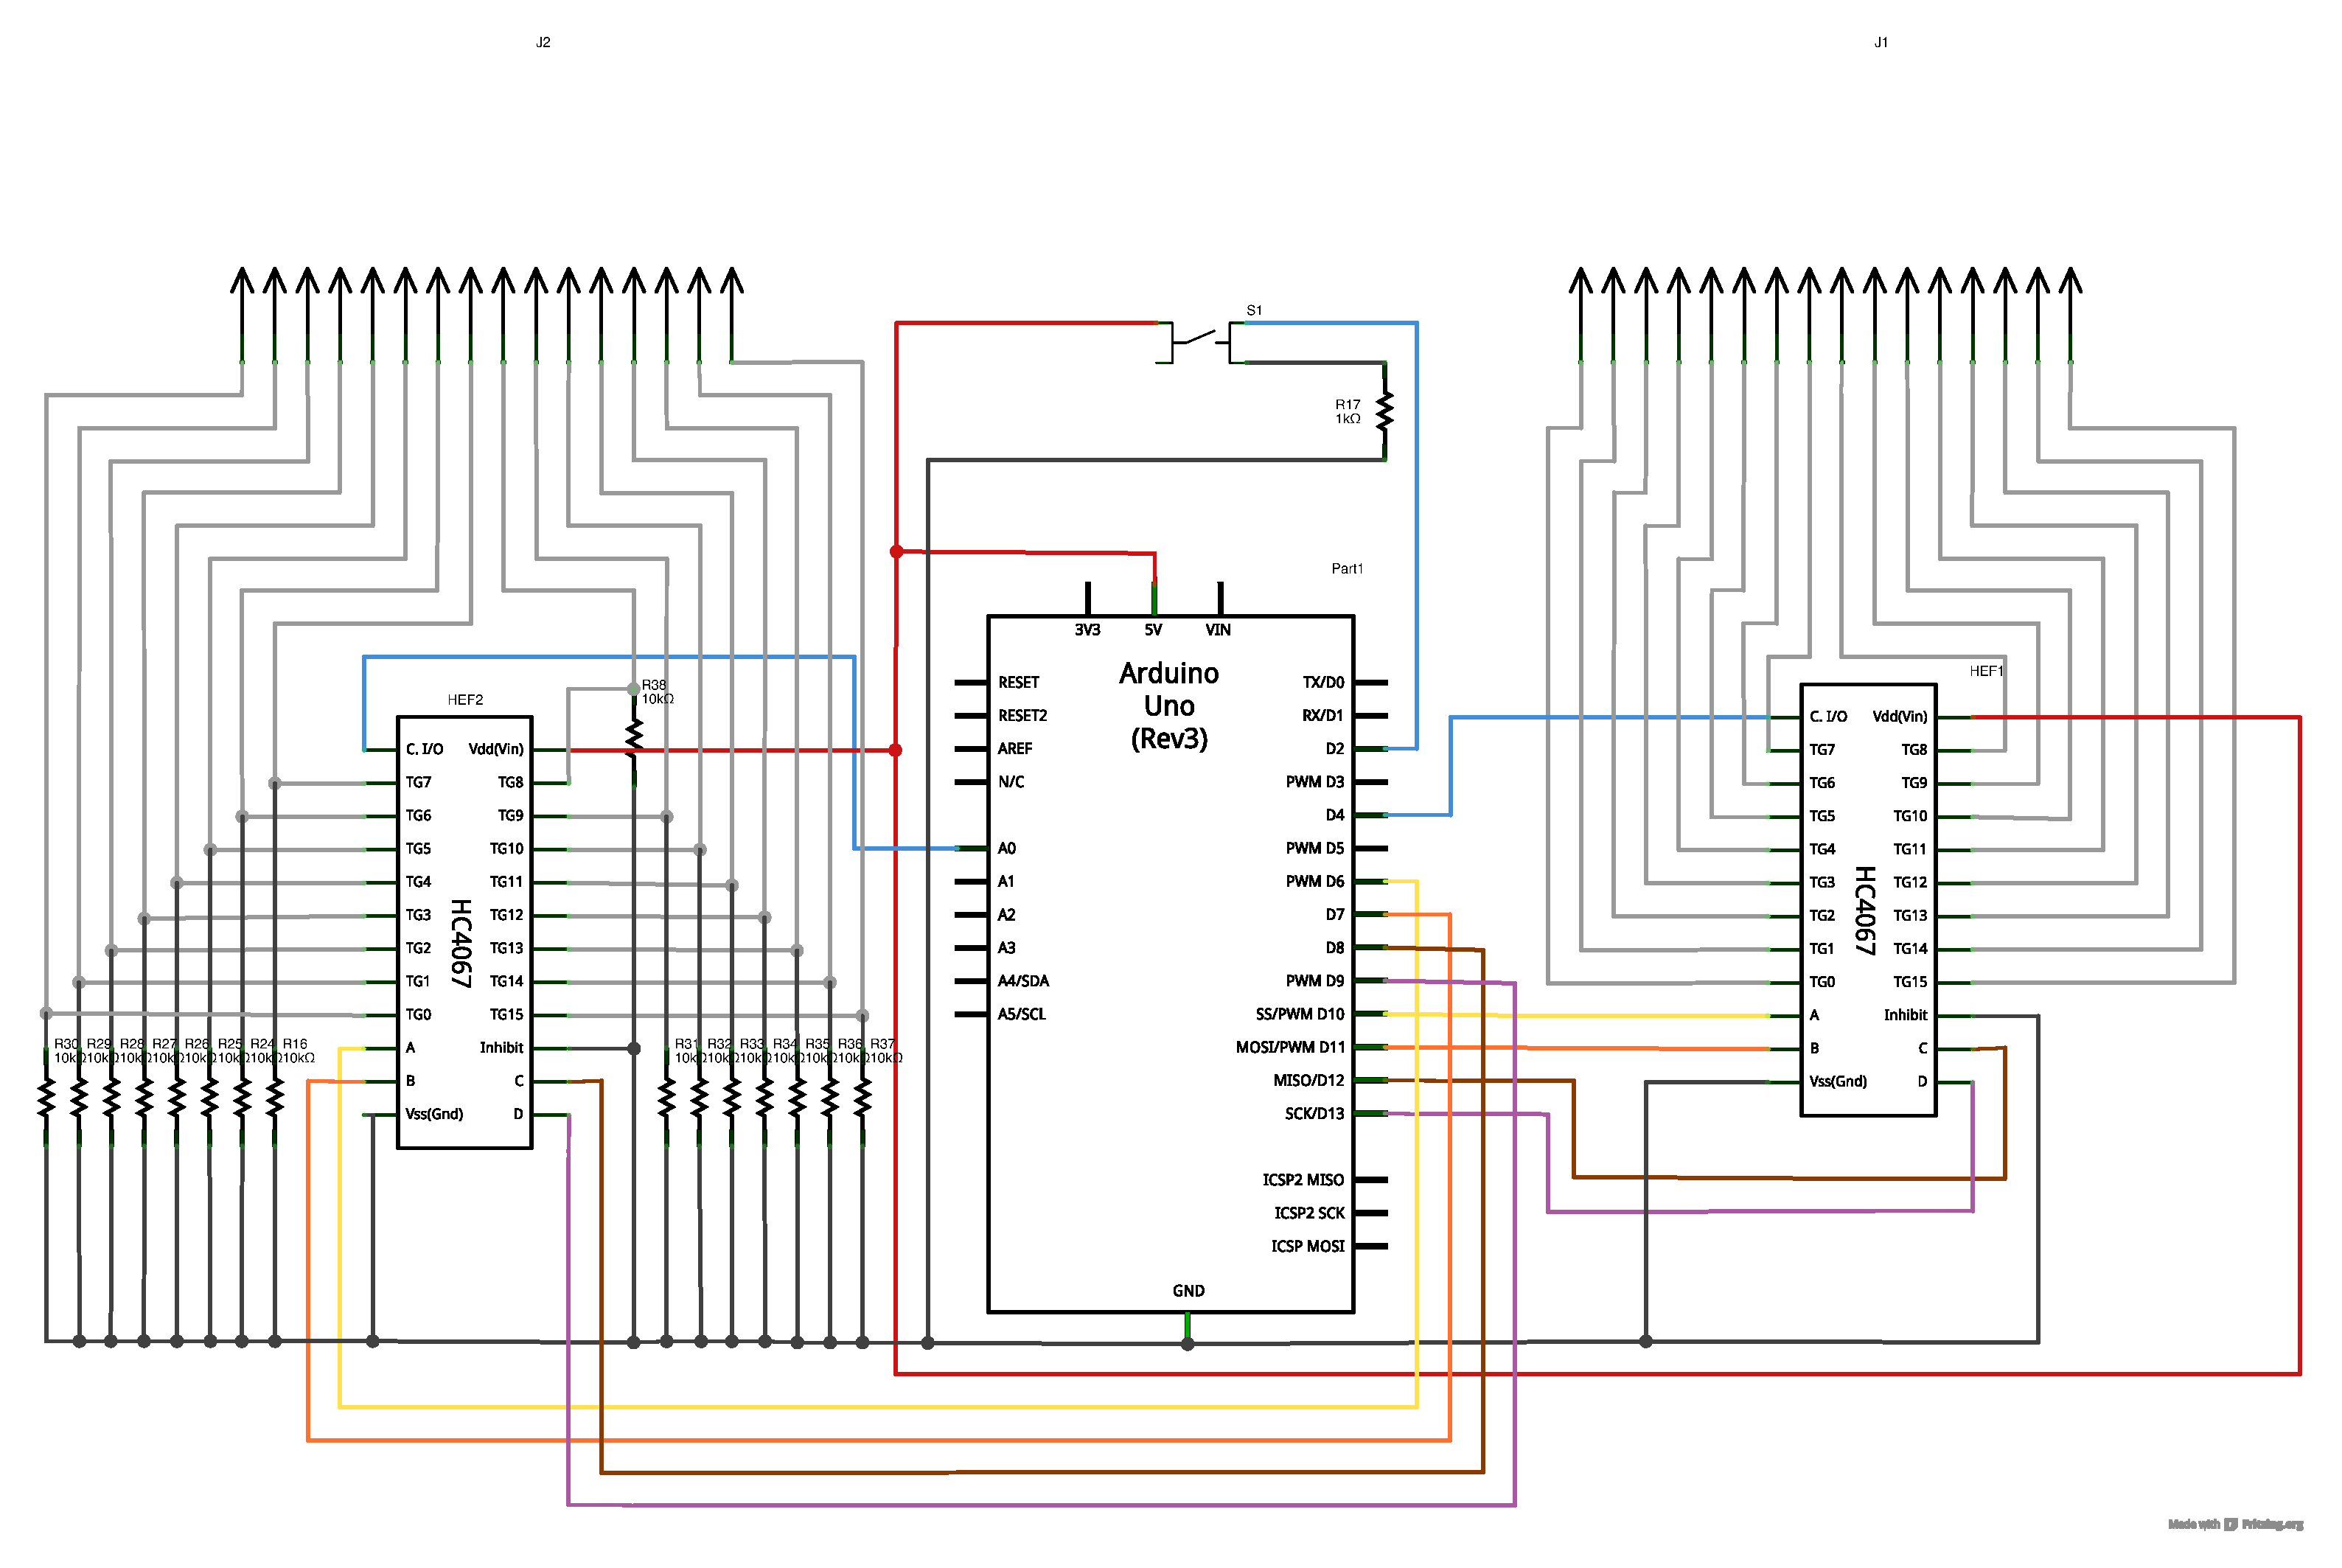
\includegraphics[width=\linewidth]{figures/schematics/textile-touch.pdf}
	    }
	    \caption{Schematic for the Textile Touch prototype.}
	\end{figure}
\end{landscape}

\begin{figure}[h]
	\centering
  		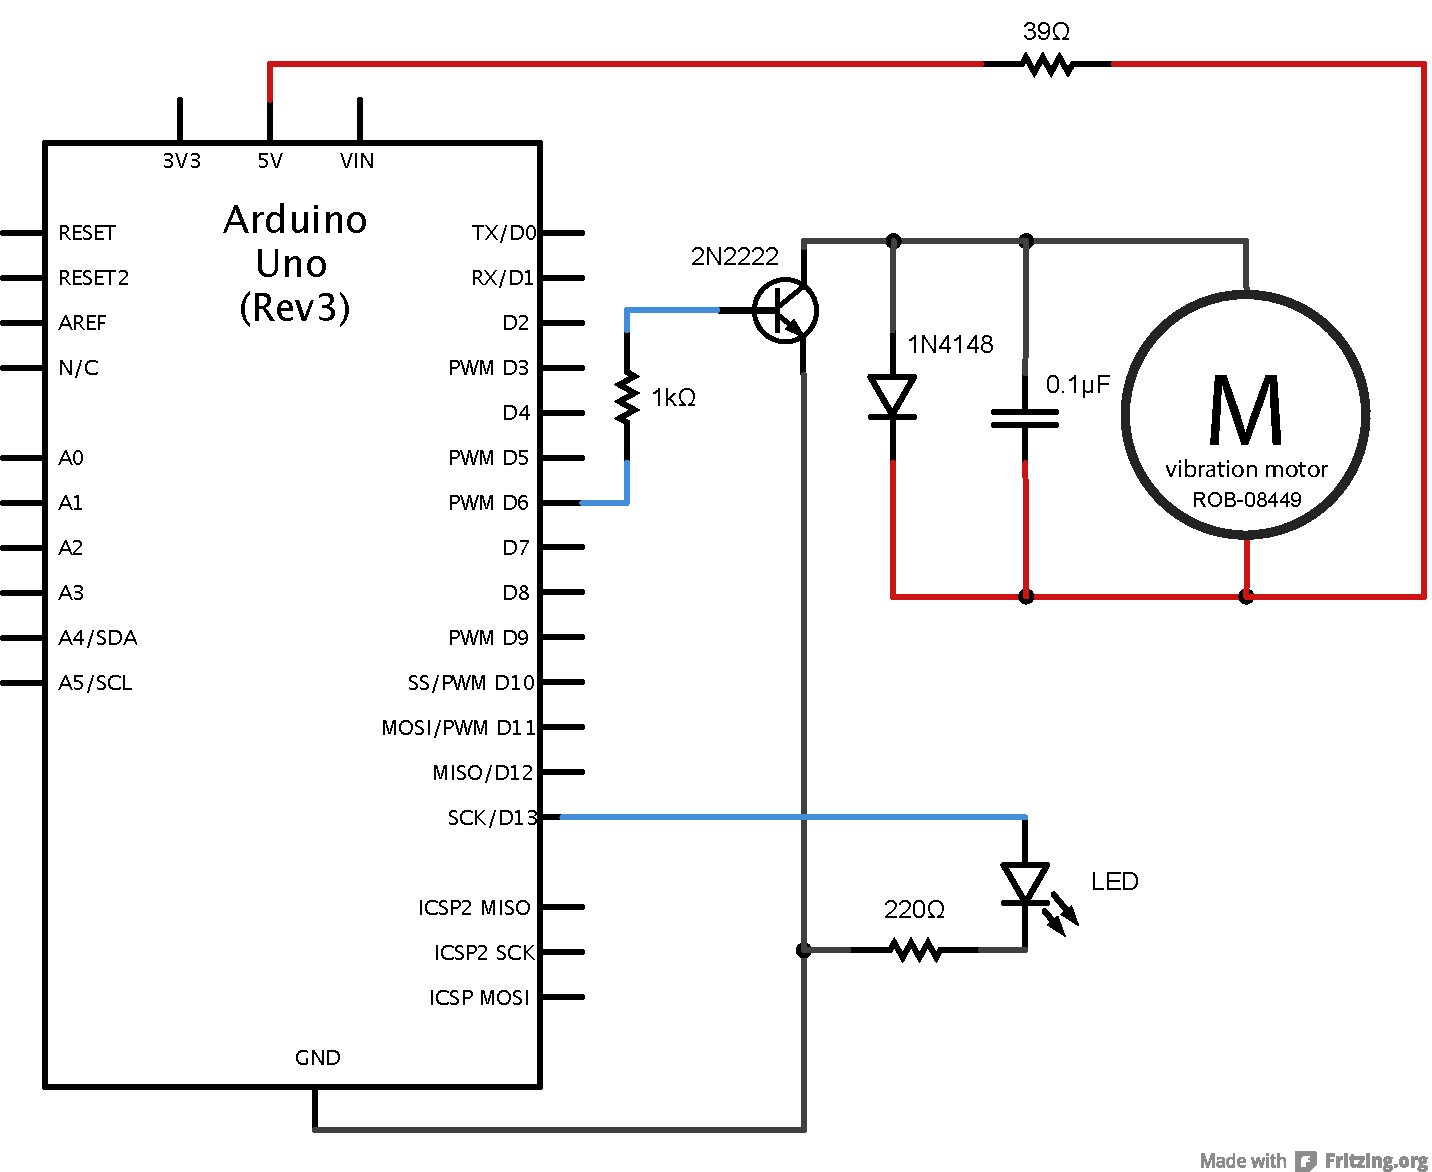
\includegraphics[width=\textwidth]{figures/schematics/textile-touch-feedback.pdf}
	\caption{Haptic and visual feedback schematic for Textile Touch.}
\end{figure}

\begin{landscape}
	\thispagestyle{empty}
	\centering
	\begin{figure}[p]
	    \makebox[\linewidth]{
	        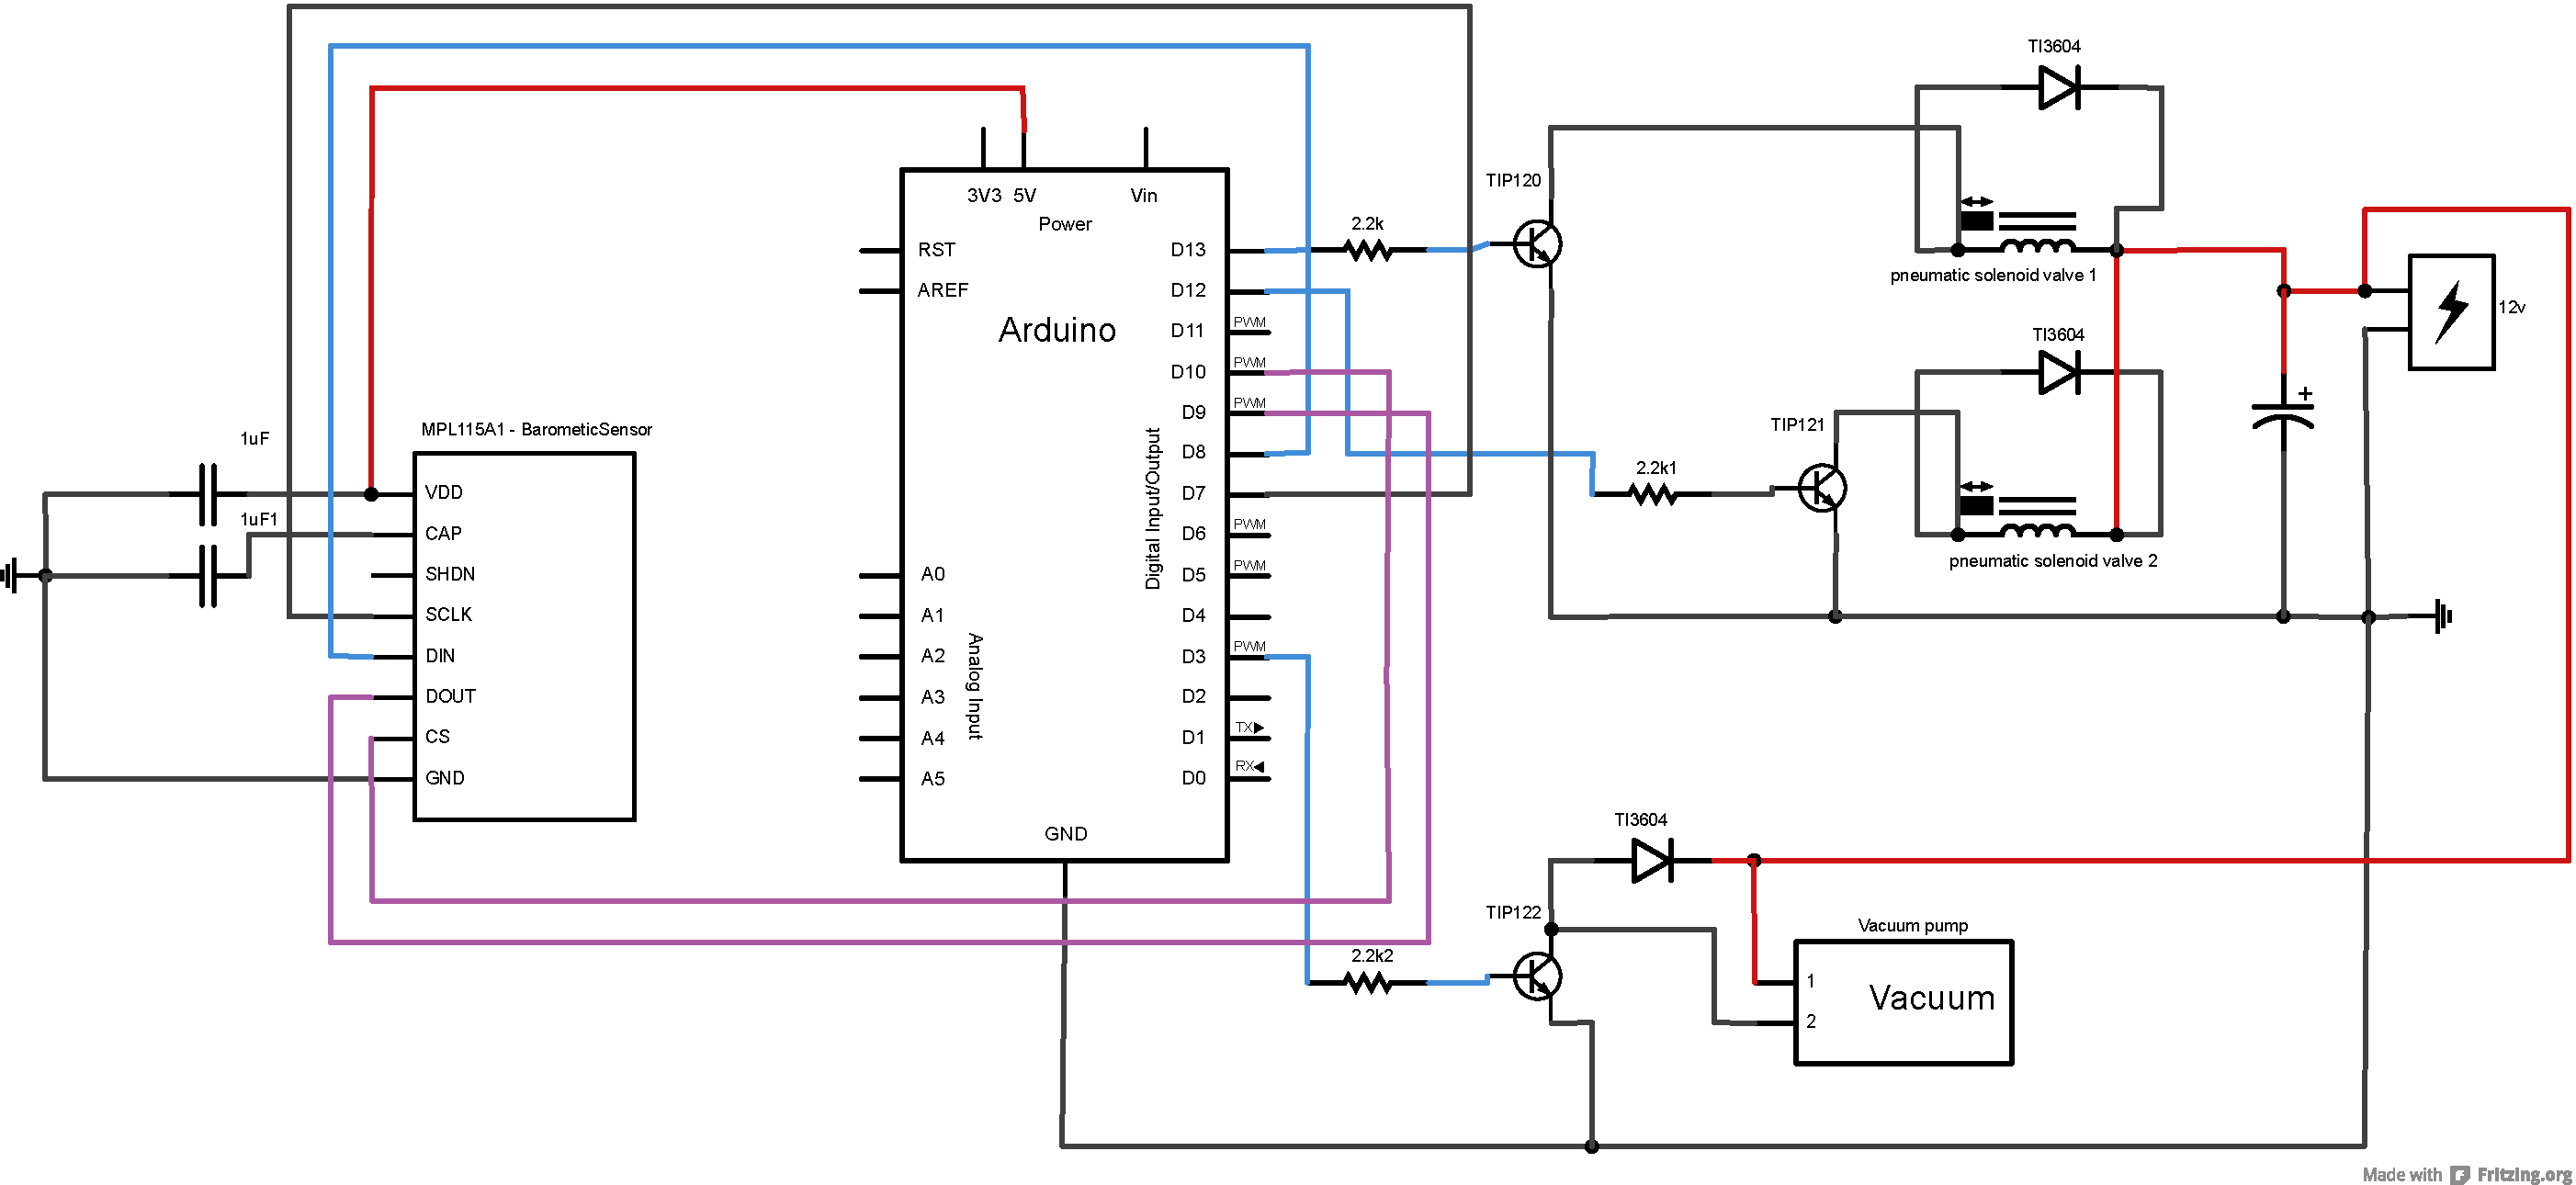
\includegraphics[width=\linewidth]{figures/schematics/jamming-draft_schem.pdf}
	    }
	    \caption{Our point of origin for a simple jamming system with a pressure sensor, two valves and a vacuum pump}
	\end{figure}
\end{landscape}